\documentclass{article}

\usepackage{summary}

\subject{Eingebettete Systeme}
\semester{Summer 2024}
\author{Leopold Lemmermann}

\begin{document}\createtitle

\section{Specification \& Modelling}

\subsection{Overview}
\subsubsection{General requirements}
\begin{enumerate}
  \item \textbf{Hierarchy}: behavioral, structural
  \item \textbf{Component-based}: esp. concurrency, communcation
  \item \textbf{Timing} (Burns, 1990): Measure time, delay, timeout, deadlines
  \item \textbf{Reactivity}: State-oriented, event-driven, exception-oriented
  \item …
\end{enumerate}

\subsubsection{Dependence graphs}
\begin{enumerate}
  \item \textbf{Directed graph}: nodes are operations/programs, edges are dependencies
  \item \textbf{Timing}: Arrival times, deadlines (for example)
  \item \textbf{I/O}: marked places
  \item \textbf{Shared resources}: small box
  \item \textbf{Periodicity}: $j_{n-1} \rightarrow j_n$
  \item \textbf{Hierarchy}: subgraphs
\end{enumerate}

\subsubsection{Models of computation and message passing}
\begin{enumerate}
  \item \textbf{Undefined components}: plain text, use cases, sequence charts
  \item \textbf{Communicating FSM} (StateCharts for shared memory): async with SDL
  \item \textbf{Data flow} (architecutre for shared memory): async with Kahn networks/SDF
  \item \textbf{Petri nets}: C/E nets, P/T nets
  \item \textbf{Discrete event model} (VHDL, Verilog, Systemc, … for shared memory): only experimental systems
  \item \textbf{von Neumann model}: C, C++, Java, …
\end{enumerate}

\subsection{Early design phase (undefined components)}
\begin{enumerate}
  \item \textbf{Plain text}: describe system in natural language
  \item \textbf{Use cases}: describe system from user perspective (possible applications), included in UML
  \item \textbf{(Message) Sequence charts (MSCs)}: describe interaction between components, included in UML
  \item \textbf{UML timing diagrams}
  \item \textbf{Life sequence charts (LSCs)}: extend MSCs with pre-charts, mandatory- vs provisional behavior
\end{enumerate}

\subsubsection{Pros \& Cons of MSCs}
\begin{itemize}
  \item[+] Appropriate for visualising schedules
  \item[+] Proved method for transporting schedules
  \item[+] Standard defined (ITU-TS)
  \item[+] Semantics defined (ITU-TS)
  \item[-] just one case, no timing tolerances
\end{itemize}

\subsection{Communicating FSMs}
see RSB/MAKS for introduction

\subsubsection{Definitions}
\begin{itemize}
  \item \textbf{Clock constraints}: conjunctive formula of atomic constraints $x-y \leq|<|=|>|\geq n\forall x,y\in C, n\in \mathbb{N}$
  \item \textbf{Timed automaton}: FSM with clock constraints
\end{itemize}

\subsubsection{StateCharts}
\begin{quote} based in shared memory computation, aggregates FSMs, allows for hierarchy, concurrency, communication, …\end{quote}

\begin{itemize}
  \item \textbf{Active states}: states with active substates
  \item \textbf{Basic states}: not composed of substates
  \item \textbf{Superstates}: composed of substates
  \item \textbf{OR-superstates} (choice): one of the substates is active
  \item \textbf{AND-superstates} (concurrency): all substates are active
  \item \textbf{History states}: remember last active substate
  \item \textbf{Timers}: special timeout edges
  \item \textbf{Edge labels}: event [condition]/action
  \item \textbf{StateMate simulation}
        \begin{enumerate}
          \item effect of external changes on events and conditions
          \item set of transitions enabled by events and right-hand side are computed
          \item transitions become active, new values for variables
        \end{enumerate}
  \item \textbf{Event lifetime}: live until step following is generated
  \item \textbf{Determinate}: given all conflicts resolved and no undefined behavior
\end{itemize}

\subsubsection{Pros \& Cons of StateCharts}
\begin{itemize}
  \item[+] arbitrary nesting of AND- \& OR-superstates
  \item[+] (StateMate-)Semantics defined
  \item[+] large number of commercial simulation tools
  \item[+] translation to SW/HW possible
  \item[-] not useful for distributed applications
  \item[-] no program constructs
  \item[-] no description of non-functional behavior
  \item[-] no object-orientation
  \item[-] no description of structural hierarchy
  \item[-] (possibly) inefficient generated programms
\end{itemize}

\subsubsection{message passing between FSMs via Specification \& Description language (SDL)}
\begin{quote} Excellent for distributed systems, asynchronous message passing, based on CFSM (like StateCharts) \end{quote}

\begin{itemize}
  \item \textbf{Process}: with State (round rectangle), Input (anti left arrow), Output (anti right arrow)
  \item \textbf{FIFO messaging}: between processes
  \item \textbf{Interaction}: process interaction diagrams
  \item \textbf{Hierarchy}: blocks, root block (system), block instance (processes cannot contain other processes)
\end{itemize}

\subsection{Data flow}

\subsubsection{Elements}
\begin{itemize}
  \item \textbf{Processes}: activites transforming data
  \item \textbf{Data stores}: holding areas for data
  \item \textbf{External entities}: sending/receiving data
  \item \textbf{Data flow}: data movement
\end{itemize}

\subsubsection{Kahn process networks (KPNs)}
\begin{quote}Components modeled as processes, connected by 1to1 FIFO channels (writes never wait, reads never block).\end{quote}

\begin{itemize}
  \item[+] processes have to commit to wait for data
  \item[+] order of reads and writes is irrelevant $\to$ determinate
  \item Turing-complete
  \item[-] timing not modeled
  \item[-] static process number
\end{itemize}

\subsubsection{Synchronous data flow (SDF)}
\begin{quote}KPN with fixed number of processes, each process has fixed number of inputs and outputs, each input/output has fixed rate.\end{quote}

\begin{itemize}
  \item[+] timing can be modeled
  \item[-] not Turing-complete
\end{itemize}

\subsection{Petri nets}
see MAKS

\subsubsection{Pros \& Cons}
\begin{itemize}
  \item[+] Appropriate for distributed applications
  \item[+] Well-known theory for formally proving properties
  \item[+] Initially a quite bizarre topic, but now accepted due to increasing number of distributed applications
  \item[-] problems with modeling timing
  \item[-] no programming elements
  \item[-] no hierarchy
  \item[ext.] enormous amounts of effort on removing limitations
\end{itemize}

\subsection{Discrete event models}

\begin{quote}Queue of future events, fetch \& execute cycle.\end{quote}
\subsubsection{Very High Speed Integrated Circuit VHSIC Hardware Description Language (VHDL)}
\begin{quote}Used for modeling digital circuits, based on Ada, used for simulation and synthesis.\end{quote}

\subsubsection{Pros \& Cons}
\begin{itemize}
  \item[+] Behavioral hierarchy (procedures and functions)
  \item[+] Structural hierarchy: through structural architectures, but no nested processes
  \item[-] No specification of non-functional properties
  \item[-] No object-orientation
  \item[-] Static number of processes, static evaluation
  \item[-] Complicated simulation semantics
  \item[-] Too low level for initial specification
  \item[$\hookrightarrow$] Good as an intermediate “Esperanto“ or ”assembly” language for hardware generation
\end{itemize}

\subsection{Imperative computation}
\begin{quote}Based on von-Neumann architecture, sequential execution, shared memory, C/C++/Java/…\end{quote}

\subsubsection{Problems with von-Neumann computing}
Mutual exclusion, holding resources while waiting for more, no preemption, circular wait.
\par $\hookrightarrow$ thread-based von-Neumann computation is inadquate for embedded systems.

\subsection{Comparison}
\begin{table}
  \centering
  \begin{tabular}{r|c|c|c|c|c}
    language    & behavioral & structural & programming & exceptions & dynamic process \\
                & hierarchy  & hierarchy  & language    &            & creation        \\
    \hline                                                                             \\
    StateCharts & +          & -          & -           & +          & -               \\
    VHDL        & +          & +          & +           & -          & -               \\
    SpecCharts  & +          & -          & +           & +          & -               \\
    SDL         & +-         & +-         & +-          & -          & +               \\
    Petri nets  & -          & -          & -           & -          & +               \\
    Java        & +          & -          & +           & +          & +               \\
    SpecC       & +          & +          & +           & +          & +               \\
    SystemC     & +          & +          & +           & -          & -               \\
    Ada         & +          & -          & +           & +          & +               \\
  \end{tabular}
  \caption{Comparison of modeling languages}
\end{table}

\subsubsection{Stuijk classification}
\begin{enumerate}
  \item expressive- \& succinctness: which systems can be modeled, how compact they are
  \item analyzability: availability of scheduling, need for run-time support
  \item implementation: required scheduling policy, code size
\end{enumerate}

There is a trade-off between expressiveness and analyzability.

\subsubsection{Mixing models}

\begin{itemize}
  \item Ptolomy \& UML: UML for structure, Ptolomy for behavior
  \item FSM/KPN in imperative languages: FSM/KPN for structure, imperative for behavior
\end{itemize}



\section{Hardware}
\begin{quote}ES hardware is, generally, used in a loop: sensing, processing, actuation.\end{quote}
\begin{figure}
  \centering
  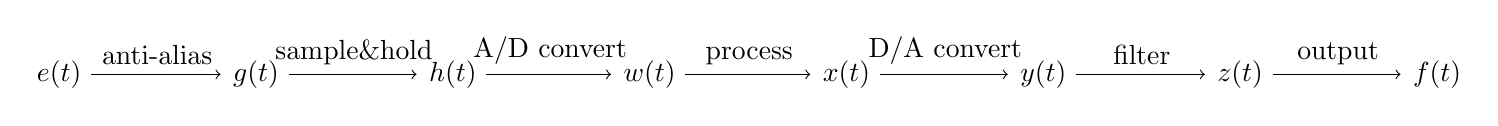
\begin{tikzpicture}[->,shorten >=1pt,auto,node distance=2.5cm]
    \node (e) {$e(t)$};
    \node (g) [right of=e] {$g(t)$};
    \node (h) [right of=g] {$h(t)$};
    \node (w) [right of=h] {$w(t)$};
    \node (x) [right of=w] {$x(t)$};
    \node (y) [right of=x] {$y(t)$};
    \node (z) [right of=y] {$z(t)$};
    \node (f) [right of=z] {$f(t)$};
    \path (e) edge node {anti-alias} (g);
    \path (g) edge node {sample\&hold} (h);
    \path (h) edge node {A/D convert} (w);
    \path (w) edge node {process} (x);
    \path (x) edge node {D/A convert} (y);
    \path (y) edge node {filter} (z);
    \path (z) edge node {output} (f);
  \end{tikzpicture}

  \caption{Signal processing chain}
\end{figure}

\subsection{A/D conversion}
\begin{itemize}
  \item \textbf{Sampling}: measure physical quantities, convert to electrical signals
  \item \textbf{Discretisation}: convert continuous signals to discrete signals
  \item \textbf{Sample-and-hold}: hold the value of the signal for a certain time
        \begin{itemize}
          \item \textbf{Nyquist theorem}: sampling frequency must be at least twice the highest frequency of the signal
          \item \textbf{Anti-aliasing}: remove frequencies above Nyquist frequency
        \end{itemize}
  \item \textbf{A/D-conversion}: convert analog signal to digital signal
        \begin{itemize}
          \item \textbf{Quantisation noise}: error due to discretisation
        \end{itemize}
\end{itemize}

\subsection{Processing}
\begin{quote}Efficiency is key: code-size, run-time, weight, cost, energy\end{quote}

\subsubsection{Energy Efficiency}
\begin{quote}Energy efficiency is the most important factor in embedded systems.\end{quote}
\begin{itemize}
  \item \textbf{Power consumption}: power supply/regulator design, interconnect dimensioning, short term cooling
  \item \textbf{Energy consumption}: restricted energy supply (mobile), cooling, thermal effects, dependability, long lifetimes
\end{itemize}

\begin{itemize}
  \item \textbf{Dynamic voltage scaling}: reduce voltage when not needed, increase when needed
  \item \textbf{Dynamic power management}: turn off parts of the system when not needed
  \item \textbf{Low \& high voltage}: with low voltage parallel, with high voltage serial more efficient
\end{itemize}


\subsubsection{Very large-scale intergration (VLSI) design}
\begin{quote}criteria: time, cost, IC properties (size, clock frequency, power consumption, …)\end{quote}

\begin{enumerate}
  \item \textbf{Full-custom design}: design every transistor, high performance, high cost, long time
  \item \textbf{Standard cell design}: use predefined cells, lower performance, lower cost, shorter time
  \item \textbf{Gate array design ($\to$ succeeded by FPGA)}: use predefined gates, low performance, low cost, short time
  \item \textbf{FPGA design}: use predefined logic blocks, low performance, low cost, short time
\end{enumerate}

\begin{table}
  \centering
  \begin{tabular}{l|ccccccc}
    Design       & performance & area & cost (IC) & cost (design) & time-to-market & process steps & quantities \\
    \hline
    Full-Custom  & +++         & +++  & +++       & - - -         & - - -          & voll          & $10^5$     \\
    Standardcell & ++          & ++   & ++        & - -           & - -            & voll          & $10^4$     \\
    Gate-Array   & +           & ◦    & +         & ◦             & ◦              & 4-10          & $10^3$     \\
    FPGA         & -           & - -  & - -       & ++            & +++            & 0             & $<10^3$    \\
  \end{tabular}
\end{table}

$\hookrightarrow$ Custom hardware is very expensive.

\subsubsection{Code-size efficiency}
\begin{enumerate}
  \item \textbf{Code compression}: reduce code size
  \item \textbf{Dictionary approach}: replace instructions with references to dictionary of frequently used instructions
\end{enumerate}

\subsubsection{Run-time efficiency}
Avoid:
\begin{itemize}
  \item \textbf{Unpredictable access to shared resources}
  \item \textbf{Branch prediction, speculative execution}
  \item \textbf{Interrupts that are possible any time}
  \item \textbf{Memory refreshes that are possible any time}
  \item \textbf{Instructions that have data-dependent execution times}
\end{itemize}

\subsubsection{Special processors}
\begin{itemize}
  \item \textbf{Very Long Instruction Word VLIW}: multiple instructions in one word, parallel execution
  \item \textbf{Explicitly Parallel Instruction Computing EPIC}: explicitly parallel instructions
  \item \textbf{Multiple Processor System on a Chip MPSoC} (also: Multi-core): multiple processors on one chip
\end{itemize}

\subsubsection{Field-Programmable Gate Array FPGA}
\begin{quote}FPGA is a chip that can be configured to implement arbitrary digital logic.\end{quote}


\begin{itemize}
  \item \textbf{Matrix of smaller logic blocks}
        \begin{itemize}
          \item \textbf{Interconnects}: Multiplexer networks
          \item \textbf{Macrocells}: Multipliers, embedded cores, …
          \item \textbf{IO-cells}: connect to the outside world
          \item \textbf{generated components}: RAM, ROM, …
          \item \textbf{Ready-made IP blocks}: processors, peripherals, …
        \end{itemize}
  \item \textbf{Complexity}
        \begin{itemize}
          \item \textbf{I/O}: ~3000
          \item \textbf{1-bit registers}: ~40 mil.
          \item \textbf{clock frequency}: ~2Ghz, 7nm
          \item \textbf{transistors}: ~92 bil.
        \end{itemize}
  \item \textbf{Producers}: Xilinx, Intel, Microchip, Lattice, Achronix, …
\end{itemize}

\subsubsection{Memory}
\begin{quote}Small is beautiful: energy consumption, access time, size\end{quote}

% TODO: add more content

\subsection{Communication}
\begin{quote}requirements: real-time behavior, efficient, economical, appropriate bandwidth \& communication delay, robustness, fault tolerance, diagnosability, maintainability, security, safety\end{quote}

\subsubsection{Robustness}
\begin{itemize}
  \item \textbf{single-ended signals}: one wire, ground reference
  \item \textbf{differential signals}: two wires, voltage difference
        \begin{itemize}
          \item[+] mostly noise immune, no effect of voltage level change, reduced importance of ground wiring, higher Speed
          \item[-] requires negative voltage, increased complexity (wires, connectors)
        \end{itemize}
\end{itemize}

\subsubsection{Real-time behavior}

\begin{itemize}
  \item \textbf{Carrier Sense Multiple Access with Collision Detection CSMA/CD}: ethernet, collision retries
  \item \textbf{Carrier Sense Multiple Access with Collision Avoidance CSMA/CA}: wifi, collision avoidance, token rings/busses
  \item \textbf{Time Division Multiple Access TDMA}: fixed time slots
  \item \textbf{Flexray}: TDMA with dynamic slots
\end{itemize}

\subsection{D/A conversion}
\subsubsection{Electrotechnical basics}
\begin{itemize}
  \item \textbf{Ohm's law}: $U = R \cdot I$
  \item \textbf{Kirchof's 1st law}: $\sum I = 0$ (current in = current out)
  \item \textbf{Kirchof's 2nd law}: $\sum U = 0$ (voltage in = voltage out)
\end{itemize}

\subsubsection{Sampling theorem}
\begin{quote}Reconstruction using sinc is precise, but not possible in practice\end{quote}

\begin{align*}
  z(t)    = & \sum_{s=-\infty}^{\infty} y(t_s) \cdot sinc(t-t_s)            \\
            & sinc(x) = \frac{\sin(\frac{\pi}{p_s}(x))}{\frac{\pi}{p_s}(x)}
\end{align*}

Limitations:
\begin{itemize}
  \item filters are only approximations
  \item all samples must be known
  \item actual signals not perfectly bandwidth limited
  \item quantisation noise can't be removed
\end{itemize}



\section{Software}

\subsection{Embedded operating systems}

\subsubsection{Requirements}
\begin{enumerate}
  \item \textbf{Configurability}: aspect-orientation, conditional compilation (preprocessor), linker-time optimisation, …
  \item \textbf{Devices handled by tasks}: use drivers directly, not through OS
  \item \textbf{Protection is optional}: SW considered reliable, protection only for safety \& security
  \item \textbf{Interrupts not OS-restricted}: any process can interrupt, no OS-protected areas (SW considered reliable)
  \item \textbf{Real-time capability}: RTOSs
\end{enumerate}

\subsubsection{Real-time operating systems RTOSs}
\begin{quote}RTOSs are designed to handle real-time requirements.\end{quote}

\begin{enumerate}
  \item \textbf{Predictability}: predictable timing behavior
  \item \textbf{Managing timing}: OS-managed timing \& scheduling
        \begin{itemize}
          \item internal synchronisation: master clock or distributed (correct with neighbors)
          \item external synchronisation: GPS is commonly used,
        \end{itemize}
  \item \textbf{Speed}: OS must be fast
\end{enumerate}

functionality: processor/memory/timer management (resources), task management, communication
classes
\begin{enumerate}
  \item \textbf{Fast proprietary kernels}: Speed over reliability $\to$ inadequate
  \item \textbf{RT extensions to general-purpose OSs}: crash of OS does not affect RT tasks, but RT-tasks cannot use OS services $\to$ less comfortable than expected
  \item \textbf{Research systems}: to avoid limitations
\end{enumerate}

\subsection{Resource access protocols}
\begin{itemize}
  \item \textbf{Priority inheritance protocol PIP}: highest priority task locks resource, lower priority task inherits priority $\to$ prevents priority inversion, but not deadlock
  \item \textbf{Priority ceiling protocol PCP}: highest priority task locks resource, lower priority task gets priority of ceiling $\to$ avoids multiple blocking
  \item \textbf{Stack resource policy SRP}: each task has a stack, if stack is full, task is blocked $\to$ dynamic priority scheduling
\end{itemize}

\subsection{(Communication) Middleware}
\begin{itemize}
  \item \textbf{Shared memory model}
        \begin{itemize}
          \item \textbf{Pthreads}: mix of hardware (shared memory) \& software (threads)
          \item \textbf{OpenMP}: parallel programming with \#pragma's, lack of control over partitioning
        \end{itemize}
  \item \textbf{Message passing model}
        \begin{itemize}
          \item \textbf{OSEK/VDX COM}: interaction layer for internal/external communication (specifies functionality, not implementation)
          \item \textbf{Common Object Request Broker Architecture CORBA}: end-to-end predictability of timeliness in fixed priority system
          \item \textbf{MPI}: asynchronous/synchronous message passing, most things explicit $\to$ lots of work, does not scale well
        \end{itemize}
\end{itemize}



\section{Validation \& Evaluation}
\begin{itemize}
  \item \textbf{Validation}: Process of determining appropriateness of a design, whether it meets constraints \& will perform as expected (yes/no decision).
  \item \textbf{Evaluation}: Process of computing quantitative information on key aspects of a design.
  \item \textbf{Verification}: Validation with mathematical rigor.
  \item \textbf{Design space evaluation}: based on Pareto points/front (trade-offs, Pareto optimality)
  \item \textbf{Criteria}
        \begin{itemize}
          \item \textbf{Average \& worst-case delay}
          \item \textbf{Power/energy consumption}
          \item \textbf{Thermal behavior}
          \item \textbf{Reliability, safety \& security}
          \item \textbf{Cost, size}
          \item \textbf{Weight}
          \item \textbf{Electro-magnetic compatibility characteristics}
          \item \textbf{…}
        \end{itemize}
\end{itemize}

\subsection{Standard optimisation techniques}

\subsection{Average \& worst-case delay}

\subsection{Power/energy consumption}

\subsection{Thermal behavior}

\subsection{Reliability, safety \& security}

\subsection{Simulation/Emulation}

\subsection{Formal verification}




\section{Mapping Applications to Platforms}


\end{document}